\documentclass{article}
\usepackage{tikz}
\usepackage{amsmath}
\graphicspath{ {images/} }
\usepackage{tocloft}
\usepackage[spanish]{babel}
\usepackage{tikz}
\usepackage{tikz-3dplot}
\usepackage[style=ieee]{biblatex}
\addbibresource{referencias.bib}


\newcommand{\myparagraph}[1]{\paragraph{#1}\mbox{}\\}

\begin{document}

\title{BORRADOR INTRODUCCIÓN TFG}

\tableofcontents
\newpage

\section{Resumen}

Desde que Hertz demostrara en 1887 la posibilidad de usar dispositivos para la transmisión de ondas electromagnéticas por un medio abierto como el aire, surgió la necesidad de poder caracterizar su comportamiento de manera fidedigna.

Con el paso del tiempo, los estándares de medida han ido evolucionando para aumentar cada vez más la precisión de la toma de medidas.  En el centro de la motivación de este trabajo está la creación de un algoritmo capaz de representar diagramas de radiación en campo lejano a partir de medidas pertenecientes al campo cercano que permita al centro de Alta Tecnología y Homologación (CATECHOM) de La Escuela Politécnica de la Universidad de Alcalá renovar el software actual de que disponen desde 1999.


\newpage

\section{Palabras clave: TO-DO} 

Acrónimos y abreviaciones 

AUT Acrónimo de antena bajo test en inglés. 

VNA Acrónimo de analizador de redes vectoriales en inglés. 

RF Acrónimo de radiofrecuencia.

FFT Acrónimo de transformada rápida de Fourier en inglés.

IFFT Acrónimo de inversa de la transformada rápida de Fourier en inglés.

DFT Acrónimo de transformada de Fourier discreta en inglés.

\newpage

\section{Introducción}
\subsection{Sobre el documento} 

El objeto principal de este trabajo es obtener un algoritmo que permita obtener
el diagrama de radiación en campo lejano a partir de las medidas del campo
eléctrico medido en la zona denominada por contra como de campo cercano
radiado por una antena.
\\

Para ello, y dado que la idea principal es poder aplicar lo estudiado en este documento sobre medidas reales, nos hemos ceñido al estándar IEEE Std-149-2021. Este es el estándar vigente a fecha de escritura de este
documento, y define todo lo referente a la toma de medidas de una antena.\\
Con su ayuda estableceremos una serie de reglas y asunciones que conviene detallar desde el principio. Por lo que esta sección introductoria servirá a este propósito.
\\

De todo lo definido por el estándar 149-2021 \autocite{IEEEstd} nos interesan dos ideas fundamentales. La primera es que vamos a centrarnos en el estudio de antenas pasivas, lineales y recíprocas. Esto implica que podemos medir sus propiedades independientemente de si durante el estudio la establecemos como transmisor o receptor.
\\

No obstante, es importante recalcar que el propio estándar afirma que gran parte de las prácticas pueden adaptarse al caso de medir sistemas que contengan elementos activos, no lineales o no recíprocos. Así, pese a que este documento ignora este tipo de sistemas, lo descrito en él podría aplicarse a dichos casos particulares.
\\
El segundo punto clave a tener en cuenta es que el estándar, y por extensión este documento, prioriza la obtención del patrón de radiación de la antena bajo estudio. Esto se debe a que es una propiedad fundamental de cualquier antena a partir de la cual podemos obtener características como la directividad, la ganancia o la eficiencia de radiación, y haciendo uso también de otras medidas disponibles en el analizador de redes con el que trabajamos.
\\
\newpage
\subsection{Sobre las instalaciones de medida}

La base principal para poder efectuar medidas sobre una antena es disponer de una instalación que cumpla una serie de requisitos muy concretos. Existen varias posibilidades válidas que satisfacen estas especificaciones. 
Esto supone que el uso de una instalación concreta determina el marco de trabajo, primando una técnica de medida sobre las demás. Motivo por el cual conviene mencionar las opciones más relevantes y centrarnos en una de ellas. 
\\

La condición ideal para medir las características de radiación del campo lejano consiste en utilizar la antena bajo estudio en modo receptor y transmitir ondas planas como radiación incidente. Recordemos que las ondas planas son ondas de amplitud constante y uniforme que presentan frentes de onda planos.\\
No obstante, en la práctica no podemos disponer de una onda plana y uniforme perfecta. Por ello, el objetivo principal a la hora de construir un espacio sobre el que tomar este tipo de medidas es poder generar una onda lo más parecida a una onda plana uniforme. 
\\

Bajo esta premisa fundamental, se idearon dos tipos básicos de instalaciones que permiten aproximarse al máximo a este tipo de ondas. 

\begin{itemize}
    \item \textbf{Las instalaciones de alcance en espacio libre} se diseñaron de forma que todos los efectos ajenos al entorno son suprimidos o llevados a niveles aceptables. Es decir, buscan simular lo mejor posible el vacío y usarlo como medio de transmisión. 
    \item \textbf{Las instalaciones de campo cercano} se idearon para poder reconstruir una onda plana uniforme. Para lo cual se hace uso de ciertas transformaciones matemáticas efectuadas sobre las muestras tomadas durante la medición. 
\end{itemize}
De entre los dos tipos de instalaciones existentes, este documento únicamente se va a centrar en las instalaciones de alcance en espacio libre. Dado que es el tipo de instalación más común y es sobre el que vamos a trabajar.\\
Dicho esto, las instalaciones de de alcance en espacio libre tienen tres subtipos de instalación principales. Las instalaciones de tipo elevada, compacta y anecoicas. De entre ellas, pondremos el foco en las instalaciones anecoicas al ser el tipo de instalación de que disponemos para tomar medidas. 

\newpage

\section{Análisis de las cámaras anecoicas}

Las cámaras anecoicas son instalaciones que se caracterizan por eliminar cualquier tipo de eco generado por una onda en su interior. Lo que hace que sean un entorno de medidas controlado y seguro que permite tomar medidas en su interior con una garantía absoluta de que no estarán contaminadas por interferencias electromagnéticas.\\

La motivación principal que impulsó la creación de estas cámaras es precisamente disponer de un entorno de medida aislado y perfectamente controlado. Dado que en un entorno abierto, las medidas se pueden contaminar por un considerablemente alto número de motivos. Entre ellos destacan la presencia de interferencias debidas a frentes de radiación externos y a las reflexiones procedentes de la antena transmisora. Además, las instalaciones abiertas están sometidas a condiciones atmosféricas que atenúan las medidas.\\
Debido a esto, el uso de la cámara anecoica se estableció como una alternativa superior a las medidas en el exterior no solo por poder eliminar las posibles interferencias, reflexiones, o por poder controlar condiciones atmosféricas que atenúan o fomenten la refracción, sino por su fiabilidad en las medidas y la facilidad con la que puede variarse la frecuencia de trabajo. De esta forma, se permite el poder caracterizar el comportamiento de una antena en un rango amplio de frecuencias de forma cómoda. Estableciendo la preferencia de este tipo de instalaciones para la medida de antenas en las que el patrón y ubicación de la fuente son factores clave. 

\subsection{Límites de las cámaras anecoicas}

Para poder trabajar adecuadamente con una cámara anecoica necesitamos conocer previamente las limitaciones que presentan este tipo de instalaciones. Existen dos factores fundamentales a nivel físico que restringen el uso de la cámara anecoica y que vienen impuestos por construcción a los cuales vamos a dedicar los siguientes dos subapartados. Estos dos factores tienen que ver con la capacidad de absorción de la cámara y las dimensiones de la misma. 

\subsubsection{Límite del absorbente de radio frecuencia }

Como hemos comentado, la eliminación del eco de las cámaras anecoicas nos permite controlar el entorno de medida eliminando las reflexiones que pueda sufrir la onda plana. Sin embargo, no hemos comentado aún nada del elemento clave que nos permite asegurar esto, el absorbente de radio frecuencia. \\

El absorbente es un elemento fundamental de las cámaras anecoicas que cobra una importancia mayor en nuestro caso en particular. Esto se debe a que la cámara anecoica de la que disponemos es del tipo rectangular, que es el modelo de cámara que más favorece la convergencia de reflexiones en la antena receptora, lo que hace que sea la cámara más sensible al rendimiento del absorbente.
\\

Para que el absorbente cumpla con su propósito de forma correcta, debemos asegurar que la impedancia presente en el espacio libre y la impedancia del propio material absorbente tengan el mismo valor o uno muy próximo. Por ello es habitual que las cámaras tengan las paredes internas recubiertas con absorbente de RF en forma piramidal, ya que gracias a esta estructura, se logra que ambas impedancias sean idénticas. 

Sin embargo, el uso de un absorbente con forma piramidal tiene como inconveniente que el rendimiento del absorbente se deteriora conforme aumenta el ángulo de incidencia de la onda sobre él. Debido a esto, es imperativo conocer el ángulo de incidencia límite a partir del cual el absorbente es incapaz de eliminar los ecos de la onda y por tanto las medidas sufren la contaminación de ondas reflejadas.\\

Este valor suele venir definido en la hoja de características del fabricante, sin embargo, es interesante conocer la variación del ángulo de incidencia límite y la capacidad de absorción conforme varía la longitud de onda. Para ello vamos a hacer uso de una gráfica que ilustra una estimación del rendimiento de un absorbente piramidal sobre el que se aplica una onda de forma oblicua definida en el estándar 149-2021 \autocite{IEEEstd}.Esta es de especial interés en nuestro caso debido a que la incidencia presente en una cámara anecoica rectangular es precisamente de tipo oblicuo. 

\newpage

\begin{figure}
    \centering
    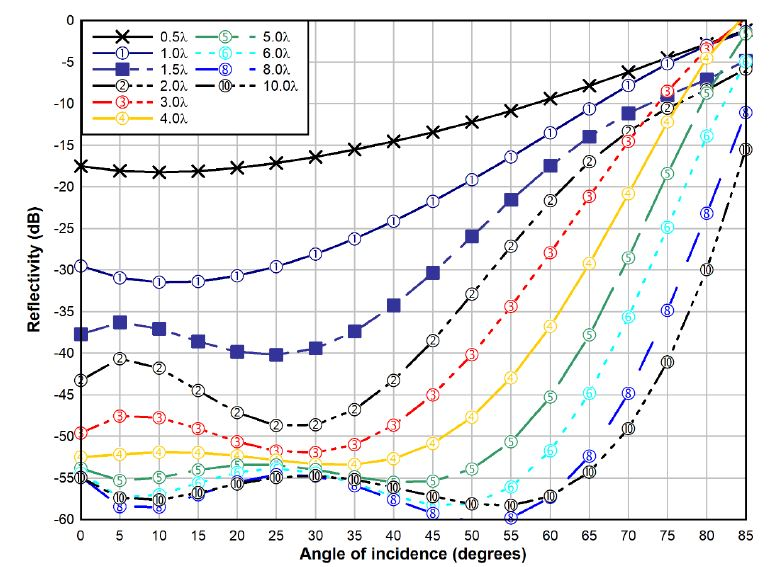
\includegraphics[scale=0.65]{Tabla-limite-angulo-incidencia}
    \caption{Curvas de la relación entre el ángulo de incidencia y la reflectividad}
    \label{Tabla-limite-angulo-incidencia}
\end{figure}

A partir de la gráfica de la figura \ref{Tabla-limite-angulo-incidencia} podemos llegar a una conclusión relativa a la longitud necesaria que debe medir nuestro absorbente. Estableciendo que, con la condición de que el absorbente sea más grande que la longitud de onda, podemos afirmar que el absorbente va a rendir correctamente y no vamos a tener ecos.
\\

Si aplicamos esta idea a un ejemplo práctico para hacernos una idea de lo que supone, significa que si empleamos una frecuencia de 150MHz perteneciente a la banda de la televisión necesitamos un absorbente que mida al menos 2 m de longitud. Estableciendo así la idea de que cuanto menor sea el tamaño de esta pirámide de absorbente, mayor será la frecuencia mínima a partir de la cual podemos efectuar mediciones sin tener efectos difractivos. 

\newpage

\subsubsection{Límite del tamaño de la cámara}

Al trabajar sobre una cámara anecoica rectangular, no solo debemos tener en cuenta el límite impuesto por el absorbente, sino también la longitud de la cámara.\\
Esto se debe a que la longitud de la cámara nos va a limitar la longitud de onda mínima que podemos usar si queremos medir una antena de tamaño concreto en nuestra cámara y utilizar esas medidas como representativas del campo lejano.\\ 

Bajo esta premisa, urge conocer la distancia a partir de la cual podemos considerar las medidas del campo como medidas del campo lejano, la cual es fácilmente obtenible a partir de la siguiente expresión: 

                            \begin{equation}
                            R =\frac{2D^2}{\lambda}
                            \end{equation}
                       
donde D es el tamaño de la apertura de nuestra antena y ${\lambda}$ es la longitud de onda en el vacío.\\
Expresión que podemos reescribir de la siguiente forma si asumimos que el tamaño de la antena será de $n$ veces ${\lambda}$.

                            \begin{equation}
                            R =2n^2\lambda
                            \end{equation}

A partir de estas expresiones podemos obtener cual es la longitud de onda máxima que podemos emplear para medir nuestra antena si conocemos cuanto mide el largo de nuestra cámara anecoica rectangular. Obteniendo de esta forma el límite de trabajo de la cámara impuesto por el tamaño de la mísma. 

\newpage

\subsubsection{Estudio de ambos límites combinados}

Una vez presentadas y explicadas ambas limitaciones, es interesante estudiar cómo se combinan entre si. Dado que nos van a marcar la frecuencia mínima y máxima que podemos usar en una cámara. 
\\

Para ello, haremos uso de la gráfica vista en la figura \ref{Tabla-limite-angulo-incidencia}. De la cual extraemos el dato de que el absorbente piramidal de altura de $2\lambda$ debe proporcionar una atenuación de 40 dB en la reflexión. 
\\

A partir de esta reflectividad; y definiendo el ángulo de incidencia $\theta$ como el ángulo límite a partir del cual el rendimiento del absorbente decae, podemos obtener la distancia a partir de la cual cumplimos el requisito de campo lejano.\\
Para encontrar dicha condición matemática, debemos aplicar relaciones trigonométricas. Por lo que hemos representado el problema a resolver en la figura \ref{Geometría-del-ángulo-incidencia-absorvente} para facilitar las cosas. 

\begin{figure}[h]
    \centering
    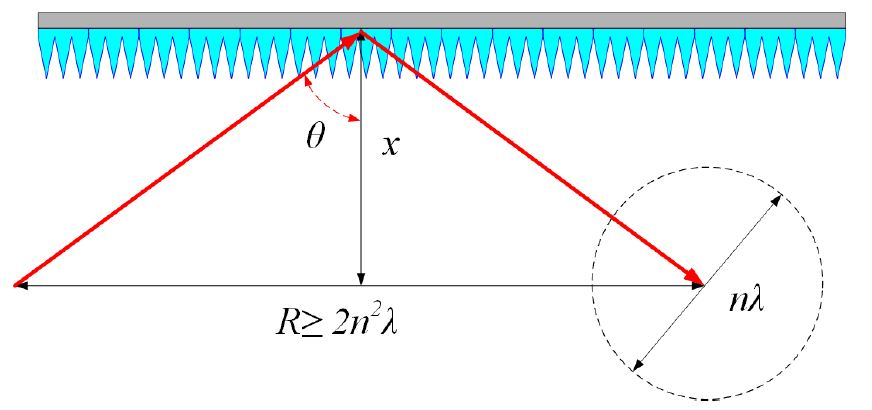
\includegraphics[scale=0.65]{Figura2-Geometria del angulo incidencia}
    \caption{Geometría del ángulo de incidencia en el absorbente de la cámara.}
    \label{Geometría-del-ángulo-incidencia-absorvente}
\end{figure}


Tras una serie de cálculos, somos capaces de obtener la siguiente expresión, que en un principio podría tomar cualquier valor: 

                        \begin{equation}
                        \tan\theta =\frac{R}{2x}
                        \end{equation}

donde x es la distancia. 

\newpage
\section{Explicación de la toma de medidas}
Tras haber dedicado una sección a comprender el tipo de instalación que vamos a utilizar y las limitaciones que implica usarla, estamos a disposición de explicar cómo se efectúa la toma de medidas dentro de una instalación.\\
En la toma de medidas, interactúan diversos sistemas de forma conjunta para poder caracterizar el comportamiento de la antena bajo test. Por ello, es interesante interesante introducir el funcionamiento de dichos sistemas y su papel en la toma de medidas. 
\\

No obstante, el objetivo de esta sección no es profundizar en cada uno de los sistemas. Lo que buscamos es presentar cada uno de los sistemas para tener un contexto de cómo es la toma de medidas dentro de la cámara.

\subsection{Arquitectura generalista de una cámara anecoica} 

Aunque previamente hemos comentado la idea de que no todas las instalaciones valen para todos los tipos de antenas, es en este punto donde debemos destacar la importancia del alcance de esta limitación.\\
Dado que los requisitos necesarios para caracterizar una antena pasiva de un solo puerto serán menos exigentes que los necesarios para medir una esfera de antenas de múltiples puertos usada para comunicaciones inalámbricas de alta velocidad. 
\\

Debido a esto; y frente a la posibilidad de tener que construir una arquitectura totalmente nueva para cada tipo de antena, se decidió plantear un modelo lo más generalista posible. El cual encontramos definido en el estándar 149-2021 \autocite{IEEEstd} y toma la siguiente forma:
\newpage

\begin{figure}[h]
    \centering
    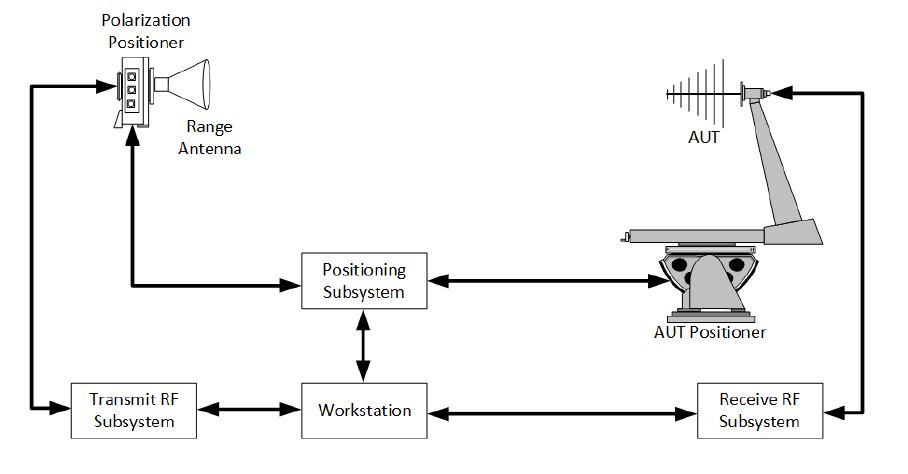
\includegraphics[scale=0.75]{Figura3-Modelo de una estacion completa de medidas}
    \caption{Esquema de una estación de medidas.}
    \label{Modelo-general-de-una-estación-de-medidas}
\end{figure}

De todos los elementos mostrados en el diagrama, solo vamos a comentar dos de ellos de forma superficial, la antena transmisora y el subsistema de posicionamiento.\\
Esto se debe a que nuestro objetivo no es detallar en profundidad cada subsistema, sino mencionar todos los aspectos clave del sistema de medición que necesitamos saber de cara a comprender las transformaciones.

\newpage

\subsubsection{Sonda} 

Si nos fijamos en la figura \ref{Modelo-general-de-una-estación-de-medidas}, vemos la aparición de un elemento sobre el que debemos hablar antes de seguir adelante, la antena transmisora.\\
Hasta ahora únicamente hemos hablado de que, idealmente, para caracterizar el campo lejano de una antena debemos radiar sobre ella una onda plana uniforme; y del hecho de que en la realidad usamos ondas semejantes debido a que no es posible generar una onda plana ideal. Pero no hemos comentamos nada relacionado con el emisor que usamos para transmitir dicha onda, que es precisamente el objeto de estudio de esta sección.
\\

El uso de esta antena, denominada sonda de ahora en adelante, es necesario para poder transmitir nuestra onda plana a la AUT y así poder obtener medidas. Lo que supone que, en aras de poder conocer el comportamiento de la antena bajo test, debemos conocer a la perfección el comportamiento de nuestra sonda.
\\

Otro concepto a destacar del uso de la sonda, es la idea de que nuestro sistema de medidas se basa en el uso de dos antenas, lo que da lugar a diferentes configuraciones posibles en función de donde se sitúan la sonda y la AUT.\\
Dándose casos donde las antenas se pueden intercambiar de posición, otros donde las dos antenas están combinadas en un mismo instrumento; y otras en las que ambas antenas están en posiciones fijas como la ilustrada en la figura \ref{Modelo-general-de-una-estación-de-medidas}..
\\

No obstante, independientemente de la configuración ante la que estemos, el funcionamiento de cada sistema es idéntico. Por lo que todo lo visto a continuación es válido independientemente de dónde estén situadas las antenas. 

\myparagraph{Frecuencia de trabajo}
A excepción de algunas instalaciones especializadas en ciertos tipos de medida, es habitual que las instalaciones de medida se diseñen para usar un rango de frecuencia lo más amplio posible que cumpla los límites aceptables de funcionamiento. Los cuales ya hemos visto cuales son y cómo calcularlos.
\\
Sin embargo, operar sobre un rango amplio de frecuencia trae consigo un problema principal. Ya que usualmente este rango de frecuencia excede el ancho de banda de trabajo de nuestra sonda. 
\\

Para solventar esto, es habitual disponer de una familia de antenas que en conjunto si permitan cubrir dicho rango de frecuencias. Lo que supone disponer de un grupo de antenas que debe tener una ganancia, ancho de haz y polarización coherentes con las medidas que queremos realizar nuestro rango.\\
Ya que no todas las antenas disponen de los mismos requisitos de línea de visión, reflexión o rangos compactos.
\\

Otro aspecto a tener en cuenta es que deseamos caracterizar la AUT en ambas polarizaciones, horizontal y vertical. Por lo que necesitamos una forma de controlar la polarización que usamos en nuestra sonda.\\
Para esto, se suele optar por usar sondas polarizadas de forma ortogonal, aunque también es habitual montar una sonda de polarización lineal sobre un posicionador de polarización. Permitiendo así orientar el ángulo de inclinación de la polarización.

\newpage

\subsubsection{Subsistema de posicionamiento} 

Para poder caracterizar una antena necesitamos tomar medidas del campo para los todos los ángulos de trabajo significativos. Lo cual es posible gracias al subsistema de posicionamiento, que es el encargado de controlar la orientación de la sonda y la AUT durante el proceso de medida.
\\

Debido a que vamos a tratar con posiciones en el espacio, es fundamental determinar el sistema de coordenadas que vamos a usar para asociar las medidas con la posición de las antenas. El cual, típicamente, es el sistema de coordenadas esféricas.
\\

Al trabajar sobre este sistema de coordenadas, independientemente de si la línea de visión es fijas o móvil, dispondremos de dos ejes ortogonales que combinados permitan efectuar cortes en $\theta$ y $\phi$. Estos ejes se designan como el eje de rotación $\theta$ y el eje de rotación $\phi$; y están representados en la siguiente figura. 

\begin{figure}[h]
    \centering
    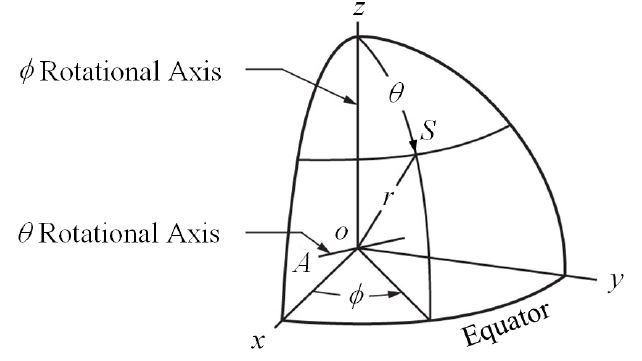
\includegraphics[scale=0.5]{Figura6-Ejes ortogonales para medir antenas}
    \caption{Ejes de rotación en un sistema esférico.}
    \label{Ejes-ortogonales-para-medir-antenas}
\end{figure} 

En nuestro caso particular, la sonda está fija y haremos pivotar la AUT de forma que podamos tomar medidas en un rango significativo de ángulos.

\newpage
\section{Transformaciones}

Todas las secciones previas servían como preparación para esta sección. Definiendo y explicando todo el contexto sobre el cual vamos a trabajar.\\
Por lo que, a partir de ahora, entraremos en profundidad en nuestro objeto de estudio siguiendo un camino natural que comienza por entender las transformaciones de puntos pertenecientes a campo cercano. De manera que, finalmente. podamos dar el salto a las transformaciones de campo cercano a campo lejano en coordenadas esféricas.

\subsection{Definición del campo cercano y lejano}

Para entender de forma simple el por qué se habla de campo cercano y lejano, debemos estudiar el comportamiento de una onda conforme se aleja de la fuente que la provocó.\\
Ya que, si pudiésemos estudiar el comportamiento de una onda electromagnética, veríamos que cuanto más se aleja de la fuente más se asemeja a un frente de ondas plano. Hasta que llegamos a un punto donde directamente podemos aproximar que la onda tiene el mismo comportamiento que una onda plana.
\\

\begin{figure}[h]
    \centering
    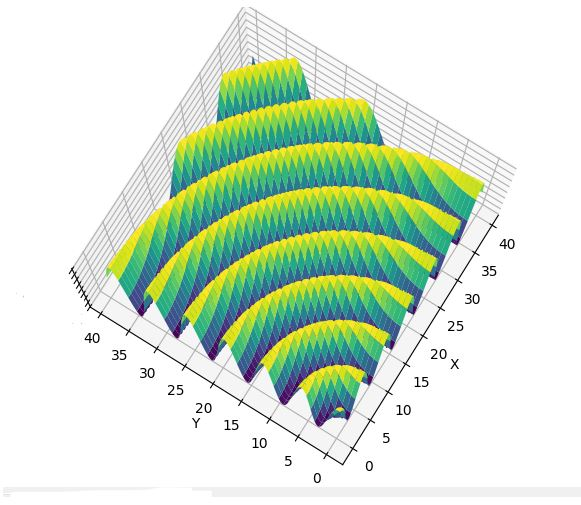
\includegraphics[scale=0.4]{Figura7-Esquema para ejemplificar el paso de onda esferica a onda plana}
    \caption{Representación visual del paso de onda esférica a onda plana}
    \label{Ejemplo-paso-onda-esferica-a-onda-plana}
\end{figure}

Precisamente es este punto en el cual la onda puede considerarse como onda plana donde se define la frontera entre campo cercano y campo lejano.\\ 
De manera que los valores del campo donde la onda aún no podemos hacer dicha aproximación decimos que pertenecen al campo cercano, mientras que aquellos valores de campo donde la onda sea próxima a una onda plana pertenecen al campo lejano. 

\newpage

En términos más exactos, el campo lejano se define como la región en la que el frente de onda saliente de una antena es plano y la variación del patrón de radiación es independiente con respecto a la distancia de la propia antena.\\
Por lo tanto, para considerar una onda perteneciente al campo lejano, su componente radial debe ser despreciable en comparación con la componente transversal; y la relación entre el campo eléctrico y magnético debe ser igual a la impedancia intrínseca del medio. Debiéndose cumplir ambos requisitos en todas las direcciones angulares vistas desde la antena.
\\

Esto supone que para determinar la distancia a partir de la cual tenemos medidas pertenecientes al campo lejano, hay que verificar estas propiedades para todas las direcciones angulares. Cosa que ocurre a una distancia igual a:

\begin{equation}
                            R =\frac{2D^2}{\lambda}
\end{equation}

donde D es la dimensión máxima de la antena y $\lambda$ es la longitud de onda de operación.\\

Si recordamos, esta fórmula ya la habíamos presentado al detallar las limitaciones presentes al usar una cámara anecoica. Lo que ilustra que, en realidad, todo el rato hemos tratado con la idea de campo lejano y campo cercano.
\newpage

\subsection{Transformación entre puntos del campo cercano}

Lo primero que debemos abordar y que nos dará una base sólida para las siguientes secciones es la transformación de un punto perteneciente a un plano $Z_1$ del campo cercano a otro plano $Z_2$ que también pertenece al campo cercano.

% Representaci ́on de los planos Z1 y Z2 en perspectiva isometrica
\tdplotsetmaincoords{60}{125} % Establecer la perspectiva
\begin{figure}[htbp]
  \centering
  \begin{tikzpicture}[tdplot_main_coords,scale=2]
    % Plano Z1 en azul
    \fill[blue!20] (0,0,0) -- (2,0,0) -- (2,2,0) -- (0,2,0) -- cycle;
    \draw[blue] (0,0,0) -- (2,0,0) -- (2,2,0) -- (0,2,0) -- cycle;
    \node[blue] at (1,1,0) {\( Z_1 \)};
    % Plano Z2 en rojo
    \fill[red!20] (0,0,1) -- (2,0,1) -- (2,2,1) -- (0,2,1) -- cycle;
    \draw[red] (0,0,1) -- (2,0,1) -- (2,2,1) -- (0,2,1) -- cycle;
    \node[red] at (1,1,1) {\( Z_2 \)};
    % Ejes
    \draw[thick,->] (0,0,0) -- (2.5,0,0) node[anchor=north east]{\( x \)};
    \draw[thick,->] (0,0,0) -- (0,2.5,0) node[anchor=north west]{\( y \)};
    \draw[thick,->] (0,0,0) -- (0,0,1.5) node[anchor=south]{\( z \)};
  \end{tikzpicture}
  \caption{Representación de los planos \( Z_1 \) y \( Z_2 \) en perspectiva isométrica.}
  \label{fig:planos_NF_Z1_Z2}
\end{figure}

Para ello, nos a basaremos en el libro \textit{Antenna Analysis and Design} de Balanis \autocite{Balanis_2016} haciendo un breve desarrollo previo que nos permita introducir de forma ordenada las ecuaciones vistas en este libro.
\\

Lo primero que debemos hacer es definir la expresión de un campo eléctrico genérico y de frecuencia $\omega$.

\begin{equation}
\vec{\tilde{E}}(\vec{r},t)=\vec{E}(\vec{r})\,e^{j\omega t}
\label{NFtoNF: eq-Campo E generico}
\end{equation}

A partir de este campo genérico, vamos a calcular su ecuación de onda lineal. Lo vual vamos a hacer aplicando el operador $\nabla^{2}$ y agregando la constante $c$ que representa la velocidad de propagación de la onda.

\begin{equation}
\nabla^{2} \vec{\tilde{E}}(\vec{r},t)=\frac{1}{c}\frac{\partial^{2}
\vec{\tilde{E}}(\vec{r},t)}{\partial t^{2}}
\label{NFtoNF: eq-de-onde-campo-electrico}
\end{equation}

Desde esta expresión, podemos llegar a la ecuación de Helmholtz basándonos en \autocite{Pozar}. Donde, aunque usan una constante $c$ menos general que la nuestra, se llega de igual forma al siguiente resultado:

\begin{equation}
\nabla^{2}+k^{2})\vec{E}(\vec{r})=0
\label{NFtoNF: eq-Helmholtz}
\end{equation}

con $k=\frac{\omega}{c}$

\newpage

Si ahora consideramos el campo $\vec{\tilde{E}}(\vec{r})$ como uno sobre el que podemos tomar medidas pertenecientes a un plano paralelo al eje $XY$ situado a una altura $z=z_{m}$ análogo a los planos vistos en la figura \ref{fig:planos_NF_Z1_Z2}, entonces la función bidimensional $\vec{E}(x,y,z=z_{m})$ se puede representar
mediante una integral de Fourier de la siguiente forma:

\begin{equation}
\vec{E}(x,y,z=z_{m})=\int_{-\infty}^{\infty}\int_{-\infty}^{\infty}\vec{\hat{E}}(k_{x},k_{y},z=z_{m})
\,e^{-j (k_{x} x+k_{y} y)} dk_{x} dk_{y}
\label{NFtoNF: eq-fourier-campo-electrico}
\end{equation}

expresión que podemos introducir en \eqref{NFtoNF: eq-Helmholtz}, obteniendo:

\begin{multline}
\left(\nabla^{2}+k^{2}\right)\left(\int_{-\infty}^{\infty}\int_{-\infty}^{\infty}\vec{\hat{E}}(k_{x},k_{y},z)
\,e^{-j (k_{x} x+k_{y} y)} dk_{x}
dk_{y}\right)=\\
\int_{-\infty}^{\infty}\int_{-\infty}^{\infty}\left(\nabla^{2}+k^{2}\right)\left[\vec{\hat{E}}(k_{x},k_{y},z)
\,e^{-j (k_{x} x+k_{y} y)}\right] dk_{x} dk_{y}=0
\label{NFtoNF: eq-fourier-campo-electrico-introducida-en-Helmholtz}
\end{multline}

donde hemos devuelto la generalidad a la componente $z$ debido a que a efecto de los cálculos puede tomar cualquier valor. Hasta ahora era específica para reforzar la relación de esta componente con los planos de medida.
\\

Si ahora operamos el Laplaciano, obtenemos:

\begin{equation}
\int_{-\infty}^{\infty}\int_{-\infty}^{\infty}\left[\left(-k_{x}^{2}-k_{y}^{2}+k^{2}\right)+\frac{\partial^{2}}{\partial
z^{2}}\right]\left[\vec{\hat{E}}(k_{x},k_{y},z) \,e^{-j (k_{x}
x+k_{y} y)}\right] dk_{x} dk_{y}=0.
\label{NFtoNF: eq-fourier-campo-electrico-introducida-en-Helmholtz-con-laplaciano-operado}
\end{equation}

como esta igualdad debe cumplirse para todos los valores de $x$ e $y$, el integrando ha de ser nulo. Lo que da como resultado:

\begin{equation}
\frac{\partial^{2}}{\partial
z^{2}}\vec{\hat{E}}(k_{x},k_{y},z)+w^{2}\vec{\hat{E}}(k_{x},k_{y},z)=0
\label{NFtoNF: resultado eq-fourier-campo-electrico-introducida-en-Helmholtz simplificada}
\end{equation}
Donde $w^{2}=k^{2}-k_{x}^{2}-k_{y}^{2}$.
\\

A partir de esta expresión, podemos definir una solución general de \eqref{NFtoNF: resultado eq-fourier-campo-electrico-introducida-en-Helmholtz simplificada} de la siguiente forma:

\begin{equation}
\vec{\hat{E}}(k_{x},k_{y},z)=\vec{\mathcal{E}^{+}}(k_{x},k_{y})\,e^{-j
w z}+\vec{\mathcal{E}^{-}}(k_{x},k_{y})\,e^{j w z}
\label{NFtoNF: solucion eq-fourier-campo-electrico-en-Helmholtz-general}
\end{equation}

donde el valor $\vec{\mathcal{E}^{+}}(k_{x},k_{y})\,e^{-j w z}$  representa una onda propagada en el sentido positivo del eje $z$, mientras que, como contrapartida, $\vec{\mathcal{E}^{-}}(k_{x},k_{y})\,e^{j w z}$ representa una onda propagada en dirección opuesta.\\

\newpage

Para nuestro caso, solamente consideraremos la solución que contiene la onda $\vec{\mathcal{E}^{+}}(k_{x},k_{y})\,e^{-j w z}$, por lo que podemos reescribir la ecuación \eqref{NFtoNF: eq-fourier-campo-electrico} teniendo en cuenta solo esta solución. Obteniendo el mísmo resultado que el visto en la ecuación (12-73) del libro de \textit{Balanis}  \autocite{Balanis_2016}.

\begin{equation}
\vec{E}(x,y,z)=\int_{-\infty}^{\infty}\int_{-\infty}^{\infty}\vec{\mathcal{E}^{+}}(k_{x},k_{y})
\,e^{-j (k_{x} x+k_{y} y+w  z)} dk_{x} dk_{y}
\label{NFtoNF:eq-fourier-balanis}
\end{equation}


\subsubsection{Algoritmo para transformar el valor del campo cercano medido en $z=z_{1}$ en el campo cercano en otro plano $z=z_{2}$}
\label{sec:Algoritmo NFtoNF}


Partiendo del desarrollo hecho en la sección anterior, estamos a disposición de generar un algoritmo que nos permitirá calcular el campo eléctrico en una posición $z$ cualquiera que no tiene por qué ser la de salida de la onda. Es decir, no tiene por qué corresponderse con el plano radiante de la antena, sino que puede ser cualquier plano posterior.\\
Esto significa que hablamos de un algoritmo capaz de calcular el campo cercano en un plano
geométrico dado por una $z$ concreta a partir de los valores del campo medido en un plano anterior.\\
Lo cual podremos hacer independientemente de si este plano pertenece a la región de campo cercano o lejano. Puesto que todo lo anterior es válido independientemente del valor de  $z$ a partir del cual consideramos que nuestro campo pasa a ser lejano.
\\

Lo primero que debemos hacer es estimar los modos dados por la función
$\vec{\hat{E}}(k_{x},k_{y},z=z_{1})$, para lo cual, hay que partir de la
ecuación \eqref{NFtoNF: eq-fourier-campo-electrico} e invertirla \footnote{En realidad, \eqref{NFtoNF:eq-fourier-campo-electrico-invertida} tiene la forma de
la transformada de Fourier directa de $\vec{E}(x,y,z=z_{1})$ como
función de $x$ e $y$, mientras que la ecuación \eqref{NFtoNF: eq-fourier-campo-electrico}
es formalmente la transformada inversa}. Lo que nos da la siguiente ecuación:

\begin{equation}
\vec{\hat{E}}(k_{x},k_{y},z=z_{1})=\frac{1}{(2\pi)^{2}}\int_{-\infty}^{\infty}\int_{-\infty}^{\infty}\vec{E}(x,y,z=z_{1})
\,e^{j (k_{x} x+k_{y} y)} dx dy.
\label{NFtoNF:eq-fourier-campo-electrico-invertida}
\end{equation}

como las medidas de las que partimos no son continuas, sino que conocemos
el campo $\vec{E}(x,y,z=z_{1})$ en un conjunto de puntos
$(x,y)=(x_{n_{x}},y_{n_{y}})$ con $n_{x}=0,1,2,\ldots,N_{x}-1$ y
$n_{y}=0,1,2,\ldots,N_{y}-1$. Deberemos discretizar \eqref{NFtoNF: eq-fourier-campo-electrico} y, por tanto,  \eqref{NFtoNF:eq-fourier-campo-electrico-invertida}. Por lo que vamos a reescribirla de la siguiente forma:

\begin{equation}
\vec{\hat{E}}(k_{x},k_{y},z=z_{1})=\frac{\Delta x
\Delta y}{(2\pi)^{2}}
\sum_{n_{x}=0}^{N_{x}-1}\sum_{n_{y}=0}^{N_{y}-1}\vec{E}(x=n_{x}\Delta
x,y=n_{y} \Delta y,z=z_{1}) \,e^{j (k_{x} n_{x} \Delta x+k_{y} n_{y}
\Delta y)}
\label{NFtoNF:eq-fourier-campo-electrico-invertida-discretizada}
\end{equation}

\newpage

A partir de \eqref{NFtoNF:eq-fourier-campo-electrico-invertida-discretizada} somos capaces de estimar los modos para cualquier valor de $k_{x}$ y $k_{y}$. Los cuales podríamos utilizar luego para calcular  \eqref{NFtoNF: eq-fourier-campo-electrico}.\\
Por lo que parece conveniente utilizar el mayor número de valores posibles y construir
una malla de puntos $(k_{x},k_{y})$ mucho mayor que la existente en $(x,y)$, que ya hemos visto que tiene $N_{x}\times N_{y}$ puntos.
\\

Sin embargo, este razonamiento presenta dos errores:
\begin{enumerate}
    \item No estamos teniendo en cuenta el teorema del muestreo dado que no por
tomar más valores de $(k_{x},k_{y})$ vamos a tener una mejor descripción
de $\vec{E}(x,y,z)$. Sino que en realidad hay un nivel de información máximo
asociado al muestreado en $(x,y)$.
    
    \item Afrontar el problema de esta forma no nos permite vincularlo con el algoritmo de la transformada rápida de Fourier (FFT). Lo que nos impide beneficiarnos de las características fundamentales de este algoritmo.

\end{enumerate}

Relativo al segundo punto, tenemos un especial interés en poder resolver nuestro problema con el algoritmo de la FFT debido a que tanto la FFT como su inversa (IFFT) son algoritmos diseñados para tener en cuenta el teorema del muestreo.
\\

Llegados a este punto es interesante estudiar brevemente ambas expresiones, por lo que vamos a comenzar definiendo la expresión de la FFT. 

\begin{equation}
\vec{\hat{E}}_{m_{x},m_{y}}=\frac{1}{N_{x} N_{y}}
\sum_{n_{x}=0}^{N_{x}-1}\sum_{n_{y}=0}^{N_{y}-1}
\vec{E}(x=n_{x}\Delta x,y=n_{y} \Delta y,z=z_{1}) \,e^{j 2\pi
\frac{m_{x} n_{x}}{N_{x}}}\,e^{j 2\pi \frac{m_{y} n_{y}}{N_{y}}}
\label{NFtoNF:eq-fft1}
\end{equation}

y a continuación la expresión de la IFFT.
\begin{equation}
\vec{E}_{n_{x},n_{y}}=
\sum_{n_{x}=0}^{N_{x}-1}\sum_{n_{y}=0}^{N_{y}-1}
\vec{\hat{E}}_{m_{x},m_{y}} \,e^{-j 2\pi \frac{m_{x}
n_{x}}{N_{x}}}\,e^{-j 2\pi \frac{m_{y} n_{y}}{N_{y}}}
\label{NFtoNF:eq-ifft1}
\end{equation}

Si compararamos  \eqref{NFtoNF:eq-fft1} con \eqref{NFtoNF:eq-ifft1}, vemos que para
poder aprovechar la herramienta que nos brinda la FFT debemos cumplir las siguientes igualdades:

\begin{subequations}
\begin{align}
k_{x}&= m_{x}\Delta k_{x}
\\
k_{y}&= m_{y}\Delta k_{y}
\\
\Delta x \Delta k_{x}&=\frac{2\pi}{N_{x}}
\\
\Delta y \Delta k_{y}&=\frac{2\pi}{N_{y}}.
\end{align}
\end{subequations}

\newpage

De todas ellas, las más relevantes para nosotros son las dos últimas debido a que son de obligado cumplimiento si queremos poder interpretar la ecuación \eqref{NFtoNF:eq-fourier-campo-electrico-invertida-discretizada} como
una FFT. Pudiendo definir\footnote{Si nos fijamos, $\Delta x$ y $\Delta y$ están
definidos por el muestreado del campo medido en $z_1$. Pero los de $\Delta k_{x}$ y $\Delta k_{y}$ aún no estaban definidos.} los valores de $\Delta k_{x}$ y
$\Delta k_{y}$ como:

\begin{align}
\Delta k_{x}&=\frac{2\pi}{\Delta x N_{x}}
\\
\Delta k_{y}&=\frac{2\pi}{\Delta y N_{y}}
\end{align}

Teniendo esto en cuenta, podemos definir la relación entre 
$\vec{\hat{E}}_{m_{x},m_{y}}$ de la ecuación \eqref{NFtoNF:eq-fft1} y 
$\vec{\hat{E}}(k_{x},k_{y},z=z_{1})$ de la ecuación \eqref{NFtoNF:eq-fourier-campo-electrico-invertida-discretizada} como:

\begin{equation}
\vec{\hat{E}}(k_{x}=m_{x} \Delta k_{x},k_{y}=m_{y} \Delta
k_{y},z=z_{1})= \Delta x \Delta y\vec{\hat{E}}_{m_{x},m_{y}}
\end{equation}

Expresión que, a nivel computacional, usaremos para calcular los modos $\vec{\hat{E}}(k_{x}=m_{x} \Delta k_{x},k_{y}=m_{y} \Delta
k_{y},z=z_{1})$ de la siguiente forma:

\begin{equation}
\vec{\hat{E}}_{m_{x},m_{y}}=\mbox{FFT}\{\vec{E}(x=n_{x}\Delta
x,y=n_{y} \Delta y,z=z_{1})\}.
\label{NFtoNF:eq-FFT-del-campo}
\end{equation}

Llegados a este punto, entramos en la segunda parte del proceso de transformación, donde haremos uso de la IFFT como herramienta para poder calcular el campo en $z=z_2$. Debiendo primero discretizar \eqref{NFtoNF:eq-fourier-balanis} de la siguiente forma para poder aproximarnos a \eqref{NFtoNF:eq-ifft1}:

\begin{equation}
\vec{E}(x,y,z=z_{2}) =
\\
\Delta k_{x} \Delta k_{y}
\sum_{m_{x}=0}^{N_{x}-1}\sum_{m_{y}=0}^{N_{y}-1} 
\vec{\hat{E}}(k_{x},k_{y},z=z_{2})
\,e^{-j(n_{x}m_{x}\Delta x  \Delta k_{x} + n_{y}m_{y}\Delta xy  \Delta k_{y})}
\end{equation}

Haciendo uso de la ecuación \eqref{NFtoNF: solucion eq-fourier-campo-electrico-en-Helmholtz-general}; y manteniendo que $\vec{\mathcal{E}^{-}}(k_{x},k_{y})=0$, entonces se cumple que:

\begin{equation}
\vec{\hat{E}}(k_{x},k_{y},z_{1})=\vec{\mathcal{E}^{+}}(k_{x},k_{y})\,e^{-j
w z_{1}}
\end{equation}

expresión a partir de la cual podemos despejar $\vec{\mathcal{E}^{+}}(k_{x},k_{y})$ como:

\begin{equation}
\vec{\mathcal{E}^{+}}(k_{x},k_{y})=\vec{\hat{E}}(k_{x},k_{y},z_{1})\,e^{j
w z_{1}}
\label{NFtoNF:Ez2-cambio-fase}
\end{equation}

Lo que finalmente nos permite calcular el campo en $z=z_2$ como:

\begin{equation}
\vec{E}(x,y,z=z_{2})=\Delta k_{x} \Delta
k_{y}\,\mbox{IFFT}\{\vec{\hat{E}}(k_{x}=m_{x}\Delta
k_{x},k_{y}=m_{y} \Delta k_{y},z=z_{2})\}.
\label{NFtoNF:Ez2-final}
\end{equation}

\newpage

Advertencias:
\begin{enumerate}
\item Como el campo es vectorial, hay que aplicar separadamente este
algoritmo a todas las componentes.
\item Por supuesto, podemos trabajar con $\Delta x=\Delta y$
\item Los dos planos y las dos rejillas de medidas tienen que tener las mismas
dimensiones pero pueden ser subdominios de áreas mayores en las
cuales, por lo que sea, eliminamos ciertos márgenes. Eso ocurre en
el caso de trabajar con medidas simuladas sobre espacios esféricos,
donde los cortes con $z$'s dados no son iguales: nos quedamos con
los subdominios de iguales dimensiones.
\end{enumerate}

\newpage
\subsubsection{Validación del algoritmo}

Una vez detallado el proceso teórico necesario para transformar las medidas del campo cercano, estamos a disposición de demostrar con un ejemplo que nuestra transformación es válida.\\
Para ello, vamos a realizar una simulación en COMSOL de una antena microsctrip  de la cual extraeremos los valores del campo cercano medido sobre un plano $Z1$ que usaremos para calcular el campo cercano en un plano posterior $Z2$.
\\

La antena microstrip que hemos construido en la simulación presenta las siguientes características básicas:

\begin{itemize}
    \item Tiene un punto de alimentación de $50\Omega$.
    \item La frecuencia de trabajo sera de 1.575 Ghz.
    \item Las dimensiones W y L de la antena son 7 mm y 15.5 mm.
\end{itemize}

\begin{figure}[h]
    \centering
    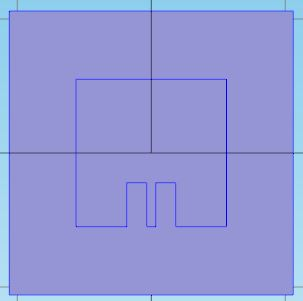
\includegraphics[scale=0.50]{Simulaciones COMSOL/MS-Planta de la antena}
    \caption{Esquemático de la antena microstrip en COMSOL.}
    \label{Simulaciones COMSOL/MS-Planta de la antena}
\end{figure}

La cual presenta el siguiente diagrama de radiación:
\begin{figure}[h]
  \centering
    \includegraphics[scale=0.45]{Simulaciones COMSOL/MS-Diagrama de radiación}
    \caption{Diagrama de radiación de la antena simulada.}
    \label{MS-Diagrama de radiación de la antena simulada}
\end{figure}

\newpage

Una vez hecha la simulación, hemos desarrollado un programa en python que implementa lo visto en \ref{sec:Algoritmo NFtoNF} utilizando los datos extraidos de la antena microstrip. No obstante, lo primero que debemos garantizar es que estamos leyendo correctamente los datos extraídos de COMSOL. Cosa que podemos verificar si enfrentamos la representación del campo a una distancia $Z1$ devuelta por COMSOL con la obtenida en nuestro programa tras leer los datos.\\

En nuestro caso, vamos a tomar las medidas del campo medido sobre el plano $Z1=15mm$ y las usaremos para obtener el campo en el plano $Z2=30mm$. Por lo que vamos a utilizar el módulo del campo en el plano $Z1$ para la comprobación, que en la simulación tiene la siguiente forma:

\begin{figure}[h] 
  \centering
    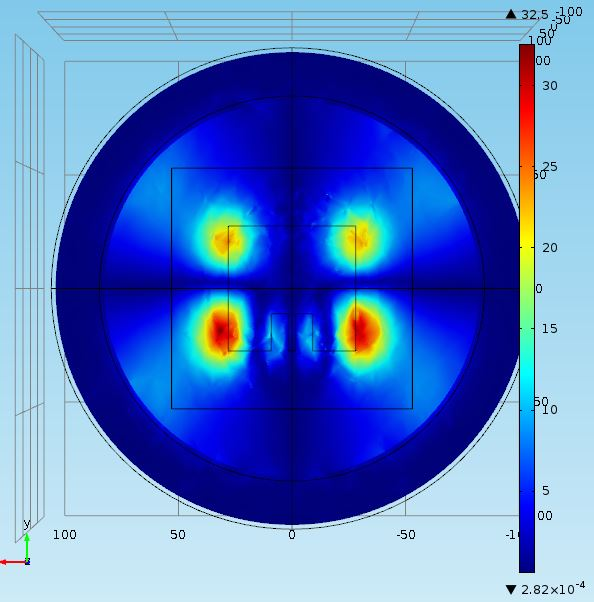
\includegraphics[scale=0.5]{Simulaciones COMSOL/MS-Enorm a 15mm}
    \caption{Módulo del campo medido en $Z1=15mm$ en COMSOL.}
    \label{MS-Diagrama de radiación de la antena simulada}
\end{figure}
\newpage

Mientras que este mismo corte representamos desde nuestro programa a partir de los datos ledos de la simulación tiene la siguiente forma:

\begin{figure}[h] 
  \centering
    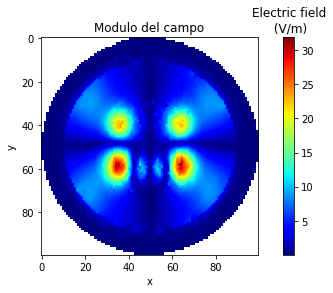
\includegraphics[scale=0.8]{Resultados python/MS-Enorm a 15mm python}
    \caption{Módulo del campo medido en $Z1$ reconstruido en python.}
    \label{MS-Diagrama de radiación de la antena simulada}
\end{figure}

Como vemos, ambas representaciones coinciden, lo que confirma que tanto el programa como la simulación trabajan con los mismos datos. Por lo que podemos realizar los cálculos que nos permiten calcular el campo en el plano posterior $Z2$ y enfrentarlos a la simulación.
\\

Cabe destacar que el propósito de esta sección es únicamente demostrar que la transformación genera valores correctos. Por lo que vamos a centrarnos únicamente en los resultados y dejar la explicación del programa para la sección \ref{sec:documentacion codigo NFtoNF}.

\newpage

El primero de los resultados que vamos a estudiar es la representación bidimensional de la FFT de las componentes cartesianas del campo. 

\begin{figure}[h] 
  \centering
    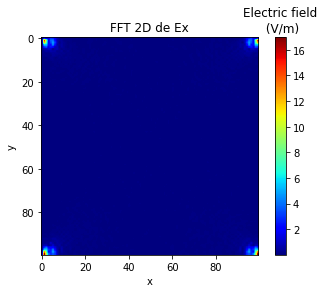
\includegraphics[scale=0.55]{Resultados python/MS-FFT 2D Ex a 15mm python}
    \caption{FFT 2D de la componente $Ex$ del campo en $Z1$}
    \label{FFT 2D Ex a 15mm}
\end{figure}

\begin{figure}[h] 
  \centering
    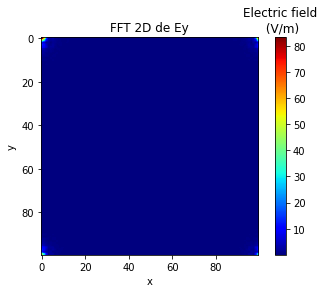
\includegraphics[scale=0.55]{Resultados python/MS-FFT 2D Ey a 15mm python}
    \caption{FFT 2D de la componente $Ey$ del campo en $Z1$}
    \label{FFT 2D Ey a 15mm}
\end{figure}

\begin{figure}[h] 
  \centering
    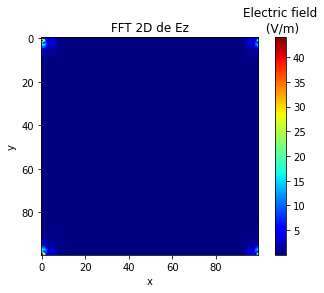
\includegraphics[scale=0.55]{Resultados python/MS-FFT 2D Ez a 15mm python}
    \caption{FFT 2D de la componente $Ez$ del campo en $Z1$}
    \label{FFT 2D Ez a 15mm}
\end{figure}
\newpage

Estas figuras corresponden al resultado de la ecuación \eqref{NFtoNF:eq-FFT-del-campo} y en ellas se muestran cuatro componentes modales situadas en las esquinas.\\
Sobre este resultado, debemos aplicar la IFFT aplicando previamente el cambio de fase tal y como veíamos en \eqref{NFtoNF:Ez2-final} y \eqref{NFtoNF:Ez2-cambio-fase}. Lo que nos devuelve los siguientes resultados:

\begin{figure}[h] 
  \centering
    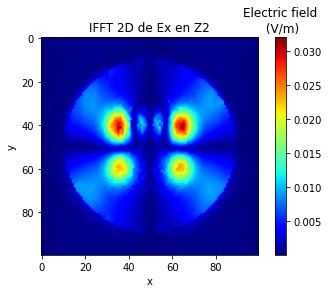
\includegraphics[scale=0.55]{Resultados python/MS-IFFT 2D Ex a 15mm python}
    \caption{IFFT 2D de la componente $Ex$ del campo en $Z1$}
    \label{IFFT 2D Ex a 15mm}
\end{figure}

\begin{figure}[h] 
  \centering
    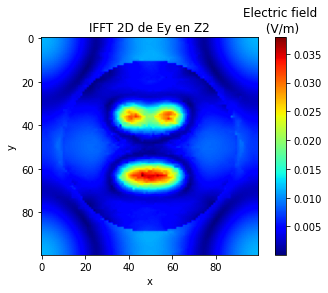
\includegraphics[scale=0.55]{Resultados python/MS-IFFT 2D Ey a 15mm python}
    \caption{IFFT 2D de la componente $Ey$ del campo en $Z1$}
    \label{IFFT 2D Ex a 15mm}
\end{figure}
\newpage
\begin{figure}[h] 
  \centering
    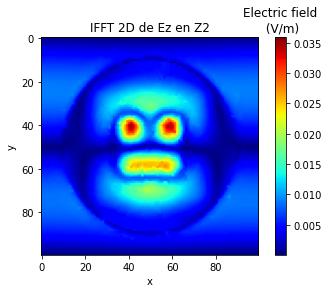
\includegraphics[scale=0.55]{Resultados python/MS-IFFT 2D Ez a 15mm python}
    \caption{IFFT 2D de la componente $Ez$ del campo en $Z1$}
    \label{IFFT 2D Ex a 15mm}
\end{figure}

\newpage

A partir de los resultados de la IFFT podemos calcular finalmente el campo en el plano $Z2=30mm$. Obtenido que su módulo en $Z2$ tiene la siguiente forma:

\begin{figure}[h] 
  \centering
    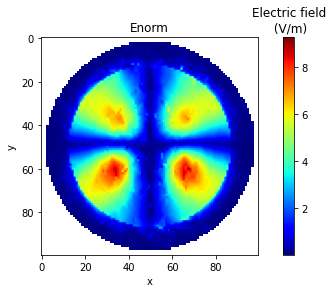
\includegraphics[scale=0.55]{Resultados python/MS-Enorm a 30mm python}
    \caption{Módulo del campo eléctrico en el plano $Z2$}
    \label{IFFT 2D Ex a 15mm}
\end{figure}

De nuevo, para verificar que este resultado es válido vamos a enfrentar esta representación del modulo con la obtenida en la simulación de COMSOL. La cual tiene la siguiente forma:

\begin{figure}[h] 
  \centering
    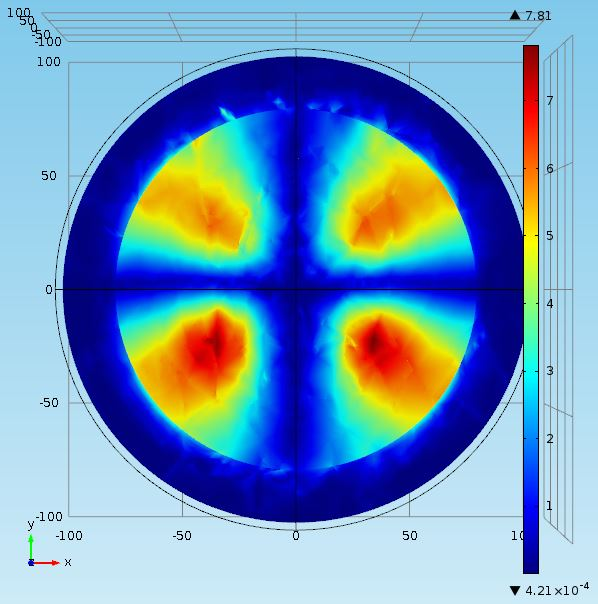
\includegraphics[scale=0.35]{Simulaciones COMSOL/MS-Enorm a 30mm}
    \caption{Módulo del campo medido en $Z2$ en COMSOL.}
    \label{IFFT 2D Ex a 15mm}
\end{figure}

Si nos fijamos, las representaciones coinciden pero los valores máximos difieren ligeramente. Esto se debe a que la escala de COMSOL sitúa los colores rojos a partir de 6 $V/m$ y la librería de python usada para representar el módulo los situa a partir de 7 $V/m$

\newpage

Una forma adicional de verificar los resultados pasa por restar los valores del módulo reconstruidos y simulados. Ya que, independientemente de la escala de color, la resta debería dar un campo prácticamente nulo como  vemos que ocurre en la siguiente figura: 

\begin{figure}[h] 
  \centering
    \includegraphics[scale=0.55]{Simulaciones COMSOL/MS-Enorm comparación cuantitativa python}
    \caption{Comparación cuantitativa del campo simulado y calculado.}
    \label{IFFT 2D Ex a 15mm}
\end{figure}

En la figura \ref{IFFT 2D Ex a 15mm} podemos ver cómo la resta de los valores pertenecientes al campo se anulan dejando una región circular central a cero mientras que los valores externos a la circunferencia presentan patrones residuales que no tienen relación con el campo surgidos de los cálculos.

\newpage

\subsection{Transformación del campo cercano medido en una superficie plana a campo lejano en coordenadas esféricas}
\label{sec:validación NFtoNF esférico}
% //Esto es una demostración de lo visto en el punto anterior. NO es una transformación.

Una vez comprendido el proceso teórico que nos permite transformar medidas entre dos planos medidos en campo cercano y tras haber validado que transformación es correcta, debemos verificar que podemos obtener las medidas del campo cercano efectuadas sobre un plano en coordenadas cartesianas y calcular con ellas las medidas pertenecientes en una superficie esférica.\\
Para ello, vamos a partir de la definición de un campo eléctrico cualquiera cuyos valores pertenecen al campo lejano.

\begin{equation}
\vec{E}(x,y,z)=\frac{jk_{z}}{2\pi r}\,e^{-jk_{0}r}{\vec{\mathcal{E}}}(k_{x}=k \sin\theta \cos\phi,k_{y}= k\sin\theta \sin\phi)
\label{NFtoFF:eq-campo-lejano}
\end{equation}

donde $k_{x}$ y $ k_{y}$  contienen la información de los ángulos del sistema de referencia esférico que sirve de base para la expresión del diagrama de radiación en el campo lejano y  $k_{z}=k\cos\theta$. Siendo $k$ el número de onda en el vacío.
\\

Para nuestra transformación, lo que realmente nos interesa es el valor del espectro, es decir, la función de modos ${\vec{\mathcal{E}}}(k_{x},k_{y})$. La cual responde a la siguiente expresión:

\begin{equation}
{\vec{\mathcal{E}}}(k_{x},k_{y})=\int_{-\infty}^{\infty}\int_{-\infty}^{\infty}\vec{E}(x,y,z=z_{0})\,e^{-j k_{x}x}\,e^{-jk_{y}y} dx dy.
\label{NFtoFF:eq-modos-del-campo-lejano}
\end{equation}
 
En la ecuación \eqref{NFtoFF:eq-modos-del-campo-lejano} podemos extraer una característica muy importante,  que la extracción de las componentes modales no depende del plano $z$, sino que puede tomar cualquier valor. Lo que significa que, mientras las medidas de dicho plano pertenezcan al campo cercano, la descomposición será siempre la misma.\\
Por otro lado, debemos tener en cuenta que en realidad solo conoceremos como es el campo  $\vec{E}(x,y,z=z_{0})$ en un conjunto discreto de puntos $(x,y) = (x_{n_{x}},y_{n_{y}})$ con  $n_{x}=0,1,2,\ldots,N_{x}-1$ y  $n_{y}=0,1,2,\ldots,N_{y}-1$. Por lo que debemos reescribir nuestra ecuación de modos para que se ajuste a este conjunto de valores a la vez que adaptamos la ecuación para que podamos hacer uso de la transformada discreta de Fourier para poder hacer uso de la FFT.

\newpage

Tras este razonamiento, vamos a reescribir la ecuación \eqref{NFtoFF:eq-modos-del-campo-lejano} de la siguiente forma: 
\begin{align}
{\vec{\mathcal{E}}}(k_{x},k_{y})&=\frac{L_{x}L_{y}N_{x}N_{y}}{4 \pi^2 (N_{x}-1)(N_{y}-1)} \nonumber \\
&\times \sum_{n_{x}=1}^{N_{x}-1}\sum_{n_{y}=1}^{N_{y}-1} DFT(\vec{E}(x=n_{x}\Delta
x,y=n_{y}\Delta
y,z=z_{0}))\,e^{-j k_{x}n_{x} \Delta x}\,e^{-jk_{y}n_{y} \Delta y}
\label{NFtoFF:eq-fourier}
\end{align}
donde:
\begin{itemize}
    \item $N_{x}$ y $N_{y}$ son respectivamente el número de puntos del campo cercano en la dirección $x$ e $y$ .
    \item $L_{x}$ y $L_{y}$  es la longitud de la apertura en las dimensiones  $x$ e $y$.
\end{itemize}

De esta forma, la ecuación \eqref{NFtoFF:eq-fourier} corresponde a la descomposición modal del campo. Sin embargo, debemos discretizando los valores de $k_{x}$ y $k_{y}$ para poder aplicar la DFT aplicando las siguientes expresiones: 

\begin{subequations}
\begin{align}
k_{x}&= m_{x}\Delta k_{x}
\\
k_{y}&= m_{y}\Delta k_{y}
\\
\Delta x \Delta k_{x}&=\frac{2\pi}{N_{x}}
\\
\Delta y \Delta k_{y}&=\frac{2\pi}{N_{y}}.
\end{align}
\end{subequations}

Cabe destacar que podemos hacer este paso debido a que hay una definición implícita de $k_{x}$ y $k_{y}$ obtenida de la teoría de la DFT y de su valor como estimador espectral. Ya que necesitamos que la multiplicación de $\Delta x \Delta k_{x}$ sea igual a $\frac{2\pi}{N_{x}}$ para poder convertir la expresión en una sobre la cual poder hacer la DFT.\\

Si volvemos al contexto de nuestras medidas, nos damos cuenta que estamos trabajando precisamente con una malla regular de valores $k_{x}\times k_{y}$ correspondientes a coordenadas cartesianas del sistema de referencia del dominio transformado. Por lo que a partir de esta malla, podemos dar una correspondencia entre los valores de $k_{x}$ y $k_{y}$ y los valores pertenecientes a una malla irregular en el dominio angular de dimensiones $\theta \times \phi$.

\newpage

Discretizando entonces los valores de $k_{x}$ y $k_{y}$ de \eqref{NFtoFF:eq-fourier} obtenemos: 

\begin{equation}
{\vec{\mathcal{E}}}_{m_{x},m_{y}}=\frac{1}{N_{x} N_{y}}
\sum_{n_{x}=0}^{N_{x}-1}\sum_{n_{y}=0}^{N_{y}-1}
\vec{E}(x=n_{x}\Delta x,y=n_{y} \Delta y,z=z_{0}) \,e^{j 2\pi
\frac{m_{x} n_{x}}{N_{x}}}\,e^{j 2\pi \frac{m_{y} n_{y}}{N_{y}}}
\label{eq-fft1}
\end{equation}

Lo que finalmente nos permite reescribir \eqref{NFtoFF:eq-campo-lejano} introduciendo el uso de los ángulos $\theta \times \phi$:

\begin{align}
\vec{E}(r,\theta,\phi)&=\frac{jk_{z}}{2\pi r}\,e^{-jk_{0}}{{\vec{\mathcal{E}}}}(k_{x}=k \sin\theta \cos\phi,k_{y}= k\sin\theta \sin\phi)\nonumber
\\
\vec{E}(r,\theta_{m},\phi_{m})&=\frac{jk_{z}}{2\pi r}\,e^{-jk_{0}}{{\vec{\mathcal{E}}}}(k_{x}=m_{x}\Delta k_{x},k_{y}= m_{y}\Delta k_{y})=\frac{jk_{z}}{2\pi r}\,e^{-jk_{0}}{{\vec{\mathcal{E}}}}_{m_{x},m_{y}}\nonumber
\\
\label{eq-fourier3}
\end{align}

Pudiendo reconstruir el campo eléctrico para cualquier valor de $\theta$ y $\phi$ a partir de esta ecuación teniendo en cuenta que los valores de los ángulos $\theta \times \phi$ pueden corresponder a valores que no formen parte de nuestra malla $k_{x}\times k_{y}$. Debiendo interpolar estos ángulos con la malla de valores  $k_{x}\times k_{y}$  para poder obtener su valor correspondiente.
\\

Advertencias:
\begin{enumerate}
\item Si efectuamos este cálculo sobre una antena bajo test, debemos saber que tiene una limitación ligada a cómo medimos físicamente la antena. Ya que solo será válido mientras respetemos ángulos de medidas menores a los siguientes:
\begin{equation}
\vartheta = \pm\arctan \frac{S-D}{2r_{0}}
\end{equation}
donde $S$ es la longitud del área de muestreo, $D$ es el diámetro de la antena bajo test y $r_ {0}$ es la distancia de separación entre la abertura de la antena bajo test y el plano de medida.
\end{enumerate}

\newpage

\subsubsection{Algoritmo para demostrar la validación}
Tras haber detallado el proceso teórico usado para demostrar que la transformación es válida, estamos a disposición de hacer una demostración práctica tal y como hicimos en el caso cartesiano.\\
Para ello, nos apoyaremos de nuevo en la simulación de la antena microstript hecha en COMSOL para extrae la información del campo medido en un plano $Z1$ cualquiera perteneciente a la región del campo cercano.\\

En esta ocasión, partiremos de las medidas tomadas en un plano $Z1 = 40mm$ para diferenciarnos del ejemplo anterior. 

\begin{figure}[h]
  \centering
    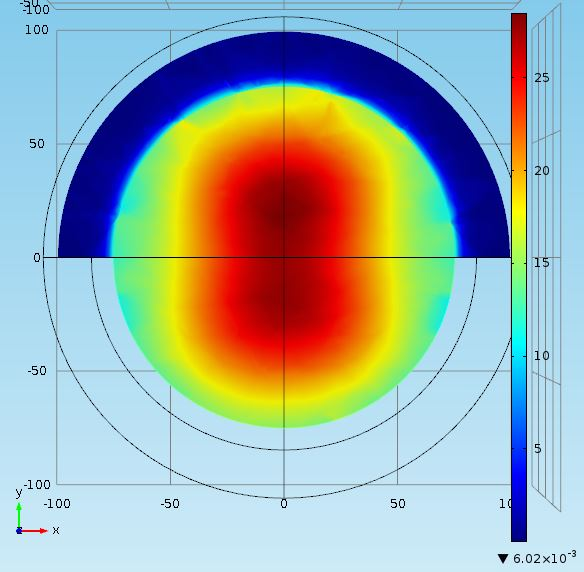
\includegraphics[scale=0.40]{Simulaciones COMSOL/MS-Enorm a 40mm}
    \caption{Módulo del campo eléctrico en $Z1 = 40m$.}
    \label{MS-Modulo del campo eléctrico en Z1}
\end{figure}

De nuevo, hemos desarrollado un programa en python que implementa lo visto en \ref{sec:validación NFtoNF esférico} partiendo de los datos extraidos de la antena microstripy que se detalla en la sección \ref{sec:documentacion codigo NFtoNF esfericas}. Por lo que en esta sección nos centraremos exclusivamente en el análisis de los resultados. \\

\newpage

Lo primero que debemos verificar es que hayamos hecho una lectura correcta de los datos tomados de COMSOL y verificar que coincide con lo visto en la figura \ref{MS-Modulo del campo eléctrico en Z1}.

\begin{figure}[h]
  \centering
    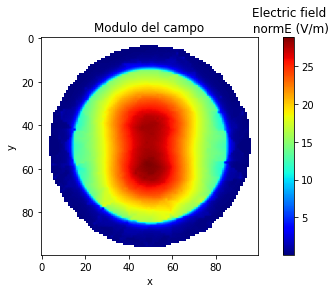
\includegraphics[scale=0.60]{Resultados python/MS-Enorm a 40mm Python}
    \caption{Módulo del campo eléctrico en $Z1 = 40m$ reconstruido en python.}
    \label{MS-MS-Enorm a 40mm Python}
\end{figure}

Si enfrentamos la figura \ref{MS-MS-Enorm a 40mm Python} con la figura \ref{MS-Modulo del campo eléctrico en Z1} vemos que efectivamente las representaciones coinciden. Confirmando de esta forma que los datos con los que vamos a tratar son exactamente iguales a los proporcionados por la simulación.\\

Tras esta comprobación, y tras procesar los datos leídos pertenecientes al plano $Z1$, estamos a disposición de emplear la FFT contando con que trabajamos con una malla regular de valores $k_{x}\times k_{y}$. Lo que supone que tendremos que dar una correspondencia entre los valores de nuestra malla y los valores pertenecientes al dominio angular de dimensiones $\theta \times \phi$.\\

\newpage

Obteniendo los siguientes valores de la FFT para cada componente del campo eléctrico:

\begin{figure}[h]
  \centering
    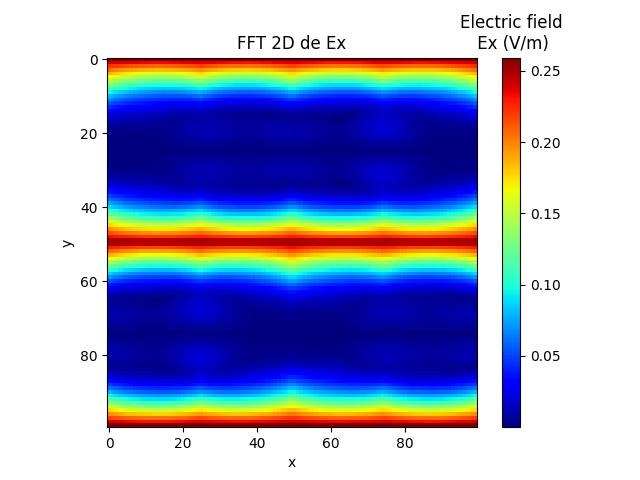
\includegraphics[scale=0.50]{Resultados python/MS- FFT 2D Ex}
    \caption{FFT 2D de la componente $Ex$ en $Z2$}
    \label{MS- FFT 2D Ex}
\end{figure}

\begin{figure}[h]
  \centering
    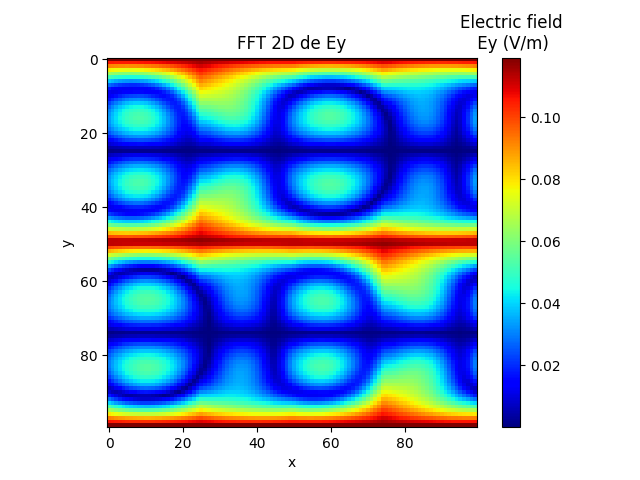
\includegraphics[scale=0.50]{Resultados python/MS- FFT 2D Ey}
    \caption{FFT 2D de la componente $Ey$ en $Z2$}
    \label{MS- FFT 2D Ey}
\end{figure}

\newpage

\begin{figure}
  \centering
    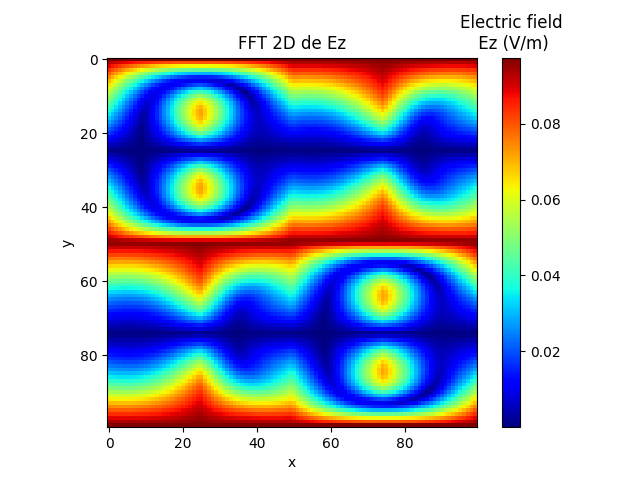
\includegraphics[scale=0.50]{Resultados python/MS- FFT 2D Ez}
    \caption{FFT 2D de la componente $Ez$ en $Z2$}
    \label{MS- FFT 2D Ez}
\end{figure}

lo que nos da la siguiente representación del módulo del campo eléctrico medido en $Z2=50mm$:

\begin{figure}[h]
  \centering
    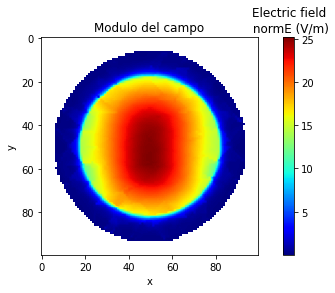
\includegraphics[scale=0.60]{Resultados python/MS-Enorm a 50mm Python}
    \caption{Módulo del campo eléctrico en $Z2$ calculado en python}
    \label{MS-FFT 2D Ez}
\end{figure}

\newpage
Que, si lo enfrentamos al valor obtenido en nuestra simulación, vemos que efectivamente coinciden:

\begin{figure}[h]
  \centering
    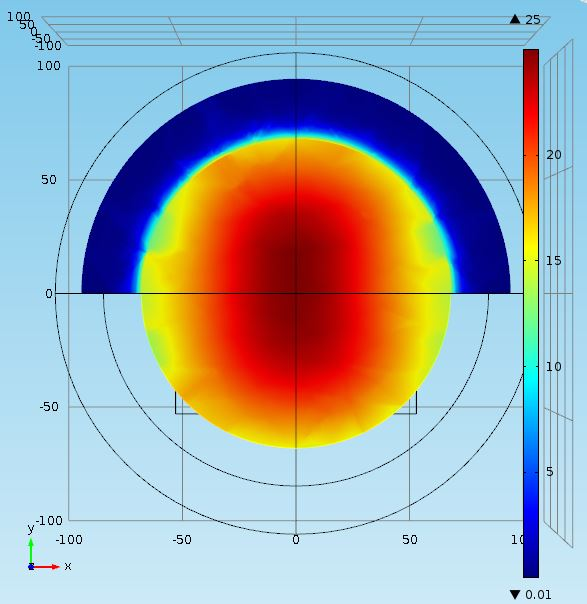
\includegraphics[scale=0.40]{Simulaciones COMSOL/MS-Enorm a 50mm}
    \caption{Módulo del campo eléctrico en $Z2$ leído de COMSOL.}
    \label{MS-Enorm a 50mm}
\end{figure}

\newpage

\subsection{Transformación del campo lejano a partir del campo cercano medido
en coordenadas esféricas}

Tras detallar las transformaciones anteriores, estamos a disposición de abordar el proceso que nos permite obtener el campo lejano a partir de medidas pertenecientes a campo cercano en coordenadas esféricas. Estableciendo como origen del sistema de coordenadas la propia antena que vamos a caracterizar.\\

Debido a que vamos a trabajar con coordenadas esféricas, vamos a tratar con ecuaciones de ondas esféricas, que son objetos matemáticos de cierta complejidad. Por lo que lo primero que debemos hacer es introducir almenos los conceptos fundamentales de estas ecuaciones.

\subsubsection{Fundamentos necesarios de las ecuaciones esféricas}

Afrontar un problema que emplea a un sistema de coordenadas curvilíneo implica que el uso de ecuaciones diferenciales presenta dificultades añadidas. \\
Por lo que, para poder reducir parte de la complejidad, vamos a apoyarnos en una característica de las ecuaciones esféricas que nos permite resolver ecuaciones diferenciales aplicadas sobre un vector (en nuestro caso, el campo eléctrico) si consideramos que podemos construir dicho vector a partir dos vectores parciales.\\

Esta propiedad solo puede aplicarse en caso de que estos vectores parciales sean derivables a partir de una función puramente escalar que satisfaga las ecuaciones de onda vectoriales. \\
En nuestro caso, siempre vamos a tratar con vectores que pueden descomponerse en vectores parciales como demostraremos en el siguiente punto. Por el momento, nos basta con saber que ciertos vectores pueden ser descompuestos en otros parciales y que este caso particular es el que nos interesa estudiar.

\subsubsection{Ecuaciones de onda vectoriales}

Como hemos dicho, la condición fundamental que permite que podamos hacer u uso de vectores parciales es que dichos vectores cumplan las ecuaciones de onda vectoriales. Motivo por el cual vamos a dedicar esta sección a presentar estas ecuaciones.\\
No obstante, las ecuaciones de onda vectoriales son, por si mismas, un objeto de estudio en si mismo. Por lo que nos centraremos únicamente en los aspectos fundamentales que son relevantes para nuestro caso de uso particular y haremos ciertas simplificaciones que iremos detallando y justificando sobre la marcha.\\

En este punto es fundamental recordar que nosotros vamos a hacer uso de una cámara anecoica para la toma de medidas que nos asegura tener un entorno de medición con unas condiciones prácticamente iguales a las del vacío.\\

\newpage

Esto significa que disponemos de un dominio cerrado, es decir, un conjunto que incluye todos sus puntos incluidos los puntos límite y cuyo complemento es un conjunto abierto. El cual además es un medio de propagación isotrópico sin fuentes.\\

Este entorno en particular resulta ser el más favorable a la hora de tratar con ecuaciones de onda vectoriales ya que todos los vectores de campo ($E$,$B$,$D$ y $H$),  el vector potencial $A$ o  los vectores de potencia de Hertz satisfacen una única ecuación diferencial que se cumple para todos ellos; y que toma la siguiente forma:
\begin{equation}
\nabla^2C - \mu\varepsilon\frac{\partial^2C}{\partial^2{t}} - \mu\sigma\frac{\partial C}{\partial{t}} = 0\
\label{eq-esfvec-general}
\end{equation}
donde $C$ representa cualquiera de los posibles vectores citados anteriormente.
\\

Partiendo entonces de esta ecuación general, lo primero que vamos a hacer es emplear la propiedad de que las ecuaciones de onda esférica son lineales. Lo que nos nos permite simplificar la implicación del tiempo de nuestra ecuación debido a que gracias a la linealidad podemos reconstruir aquellos vectores que tengan una variación arbitraria con el tiempo a partir de soluciones armónicas. Pudiendo de esta forma reescribir la ecuación \eqref{eq-esfvec-general} sin perder con ello la generalización presente en expresión. \\

Esto implica que podemos afirmar que nuestro vector $C$ únicamente varía con respecto al tiempo en base al factor $e^{-jwt}$. Cosa que nos permite simplificar aún más nuestra expresión si recordamos que el operador laplaciano ($\nabla^2$) aplicado sobre un vector cualquiera equivale a:
\begin{equation}
\nabla^2C =\nabla\nabla C - \nabla\times\nabla\times C + k^2C
\label{eq-nabla-sobre-vector}
\end{equation}
con $k^2$ = $\mu\varepsilon w^2 + j\mu\sigma w$ .\\

Si aplicamos todo lo anterior, podemos entonces reescribir  \eqref{eq-nabla-sobre-vector} de la siguiente forma:
\begin{equation}
\nabla\nabla C - \nabla \times \nabla \times C + k^2 C = 0
\label{eq-esfvec-simplificada}
\end{equation}

\newpage

Una vez hemos llegado a la ecuación \eqref{eq-esfvec-simplificada}, disponemos de dos alternativa para trabajar con ella: 

\begin{enumerate}
    \item Podemos resolver \eqref{eq-esfvec-simplificada} como un sistema de tres ecuaciones escalares.
    \item Podemos simplificar la resolución de \eqref{eq-esfvec-simplificada} resolviendo tan solo tres ecuaciones escalares independientes si y solo si podemos obtener $C$ a partir de sus componentes rectangulares.
\end{enumerate}

De estos dos métodos, siempre vamos a preferir el segundo debido a que la resolución del sistema de ecuaciones implica una alta complejidad en los cálculos. Lo cual es especialmente desfavorable si lo comparamos con la resolución de las tres ecuaciones independientes.
\\

En nuestro caso particular podemos aplicar el segundo método debido a que siempre vamos a ser capaces de obtener el campo medido a partir de sus componentes rectangulares ya que nuestras medidas siempre van a cumplir las propiedades de ortogonalidad.\\
Por lo que, llegados a este punto, podemos reescribir \eqref{eq-esfvec-simplificada} de la siguiente manera:

\begin{equation}
\nabla^2C_{j} + k^2C_{j} = 0
\label{eq-nabla-cuadrado-coordenada}
\end{equation}

donde $C_{j}$ hace referencia las componentes ($x$,$y$,$z$) del vector $C$.
\\

Esto significa que tendremos tantas soluciones de \eqref{eq-nabla-cuadrado-coordenada} como vectores $C$ existan. Por lo que de ahora en adelante vamos a considerar $\psi$ como una función escalar cualquiera que es solución de \eqref{eq-nabla-cuadrado-coordenada} para representar dicha generalidad.

\begin{equation}
\nabla^2\psi + k^2\psi = 0
\label{eq-nabla-cuadrado-coordenada-con-una-soculicon-por-vector-C}
\end{equation}

De esta forma; y considerando  '$a$' como un vector unitario constante cualquiera, podemos escribir tres vectores independientes a partir de $\psi$ que son, de hecho, solución de \eqref{eq-esfvec-simplificada}:
\begin{subequations}
\begin{align}
    L&= \nabla\psi \label{eq:Lirrotacional}\\
    M&= \nabla\times a\psi\\
    N&=\frac{1}{k}\nabla\times N
\end{align}
\end{subequations}

Estas tres ecuaciones presentan ciertas propiedades que merece la pena destacar. De entrada, gracias a ser '$a$' un vector unitario, podemos reescribir $M$ de la siguiente manera:    

\begin{equation}
M= L \times a = \frac{1}{k}\nabla \times N
\label{eq-M-reescrito}
\end{equation}

\newpage

Por otro lado, el vector $M$ es perpendicular a $L$ para nuestra posible solución $\psi$, lo que significa que $L\cdot M=0$.Mientras que, por definición, $L$ cumple las siguientes dos propiedades:
\begin{align}
    \nabla  \times L &=0 \\
    \nabla  \cdot L  &=\nabla^2\psi = -k^2 \psi
\end{align}

donde hemos aplicado la ecuación \eqref{eq:Lirrotacional} para obtener el carácter rotacional del vector $\vec{L}$ y convertir su divergencia en un laplaciano.
\\

Si además de lo anterior tenemos en cuenta que $M$ y $N$ son vectores de campo eléctrico en nuestro caso particular, significa que tanto $M$ como $N$ son capaces de crear un campo magnético. Por lo que, como pertenecen a un dominio que podemos considerar prácticamente igual al vacío, sus divergencias son nulas para cualquier punto dentro de él, o lo que es lo mismo, los vectores $M$ y $N$ cumplen la condición de campo solenoidal:
\begin{align}
    \nabla\cdot M &= 0
    \label{M-cumplen-ser-campo-solenoidal}\\
    \nabla\cdot N &= 0
    \label{N-cumplen-ser-campo-solenoidal}
\end{align}


Una vez presentadas todas estas propiedades de los vectores $L$, $M$ y $N$, hay que tener en cuenta que existen tres tipos de soluciones para una ecuación diferencial, la general, la particular y la singular.\\
En nuestro caso concreto, podemos asumir que para cada punto existe una única solución $C$ correspondiente al valor del campo eléctrico en dicho punto. Lo que significa que vamos a manejar las soluciones particulares de \eqref{eq-nabla-cuadrado-coordenada-con-una-soculicon-por-vector-C}. \\
Para ilustrar esto, de ahora en adelante vamos a hacer uso de la notación $\psi_{n}$ para hacer referencia a cualquiera de estas soluciones particulares de la ecuación diferencial. De forma que para cada solución $\psi_{n}$ existe un conjunto de vectores $L_{n}$, $M_{n}$ y $N_{n}$.\\

Es importante diferenciar esta generalidad de la anterior, ya que ahora no nos estamos refiriendo a una ecuación general $\psi$ sino a $\psi_{n}$ soluciones de ecuaciones que podemos obtener debido a que cumplen con los puntos anteriores que nos permiten asumir que existe una única solución para cada punto obtenible a partir de sus vectores $L_{n}$, $M_{n}$ y $N_{n}$.
\\

De los tres vectores $L_{n}$, $M_{n}$ y $N_{n}$ solo vamos a trabajar con $M_{n}$ y $N_{n}$ debido a que a cuando tratamos con una función solenoidal, es decir, una función cuya divergencia es nula en todo el dominio de puntos en la que existe dicha función, su extensión se puede obtener únicamente en términos de  $M_{n}$ y $N_{n}$.\\
Lo que supone que a partir de los vectores parciales $M_{n}$ y $N_{n}$ podemos obtener el valor del campo.\\

\newpage

Todo esto significa que si se cumple que:
\begin{enumerate}
    \item Que la variación arbitraria del tiempo entra en juego únicamente como un factor armónico $e^{-jwt}$.
    \item Que estamos trabajamos con un medio donde la densidad de cargas libres es nulo en todas partes.
    \item   Que nuestro medio es isotropico.
    \item Podemos caracterizar la conductividad de nuestro medio de forma única con valor $\sigma$.

\end{enumerate}

entonces podemos definir los campos $E$ y $H$ de esta forma:

\begin{equation}
E = \frac{jw\mu}{k^2}\nabla \times H\xrightarrow{}   H= \frac{1}{jw\mu}\nabla \times E
\label{campo-EyH-cumpliendo-simplificacion-con-MnyNn}
\end{equation}

Si suponemos además que el vector potencial también puede ser representado por una expansión de funciones vectoriales características, entonces podemos escribir el valor del vector potencial como:

\begin{equation}
A = \frac{1}{w}\sum_{n}(a_{n}M_{n}+b_{n}N_{n}+c_{n}L_{n})
\label{vector-potencial-cumpliendo-simplificacion-con-MnyNn}
\end{equation}

donde los coeficientes $a_{n}, b_{n}, c_{n}$ pueden ser obtenidos a partir de la distribución de carga del campo.
\\

Siendo en este punto donde vamos a aplicar las propiedades de $L_{n}$, $M_{n}$ y $N_{n}$ mencionadas anteriormente para poder ignorar el vector $L_{n}$. De manera que haciendo uso de la relación $\mu H = \nabla \times A$ podemos escribir las ecuaciones de campo como:


    \begin{equation}
        E = - \sum_{n}(a_{n}M_{n}+b_{n}N_{n})
    \label{eq-E general usando Mn y Nn}
    \end{equation}

    \begin{equation}
         H = - \frac{k}{jw\mu}\sum_{n}(a_{n}M_{n}+b_{n}N_{n})
    \label{eq-H general usando Mn y Nn}
    \end{equation}  


Por lo que a partir de \eqref{eq-E general usando Mn y Nn} somos capaces de expresar nuestro campo eléctrico en función de las ecuaciones de onda esférica $M_{n}$ y$N_{n}$ y los coeficientes de onda $a_{n}$ y $b_{n}$. Pudiendo entonces definir una expresión que obtenga el campo eléctrico para cualquier valor de $r$, $\theta$ y $\phi$ de la siguiente forma:
\begin{equation}
\vec{E}(r,\theta,\phi)=\sum_{n=-Nm}^{Nm}(a_{n}M_{n}(r,\theta,\phi)+b_{n}N_{n}(r,\theta,\phi))
\label{eq-campoE-coordenadas-esfericas}
\end{equation}
\newpage
\subsubsection{Método para la obtención del campo lejano}
Hasta ahora hemos hecho referencia a campos. Pero lo que realmente va a interesarnos a partir de ahora es el estudio de los  modos del campo eléctrico.\\
Es por esto que debemos mencionar el desuso  del subíndice  $n$ que hemos venido usando hasta ahora para representar que tratábamos con soluciones particulares de la ecuación diferencial.\\
Ya que a partir de ahora, vamos a referirnos siempre a modos, por lo que usaremos el subíndice $m$ y $n$ para ello.\\

Es por esto por lo que de ahora en adelante, en lugar de usar la ecuación del campo eléctrico definida en \eqref{eq-campoE-coordenadas-esfericas}, vamos a reescribirla para poder obtener $\vec{E}(r,\theta,\phi)$ a partir del desarrollo de sus modos:
\begin{equation}
\vec{E}(r,\theta,\phi)=\sum_{m=-M}^{M}\sum_{n=-N}^{N}\big[a_{n}M_{mn}(r,\theta,\phi)+b_{n}N_{mn}(r,\theta,\phi)\big]
\label{eq-campoE-coordenadas-esfericas-a-partir-de-sus-modos}
\end{equation}

TO-DO

\newpage
\section{Documentación códigos python [NOMBRE TEMPORAL]}

En esta sección se pretende documentar el código python usado para hacer las transformaciones. Detallando los diferentes programas desarrollados en sus respectivos apartados.

\subsection{Algoritmo de la transformación campo cercano a campo cercano en cartesianas}
\label{sec:documentacion codigo NFtoNF}

Esta sección recoge la documentación del código empleado para demostrar la transformación de campo cercano a campo cercano en coordenadas cartesianas.

\newpage

\subsection{Algoritmo de la transformación campo cercano a campo cercano en esféricas}
\label{sec:documentacion codigo NFtoNF esfericas}

El algoritmo utilizado para hacer esta transformación responde al siguiente diagrama de flujo:

\begin{figure}[h]
  \centering
    \includegraphics[scale=0.60]{draw io/Esquema codigo NFtoNF Esférico}
    \caption{Diagrama de flujo del código.}
    \label{DWIO:NFtoNF esfericas}
\end{figure}

Por lo que detallaremos cada uno de estos apartados por separado.
\newpage
\subsubsection{Lectura de ficheros}

Debido a que este programa pretende únicamente demostrar la transformación, está orientado a leer únicamente los ficheros proporcionados por COMSOL. Lo que significa que trataremos con ficheros que siguen la siguiente estructura:

\begin{figure}[h]
  \centering
    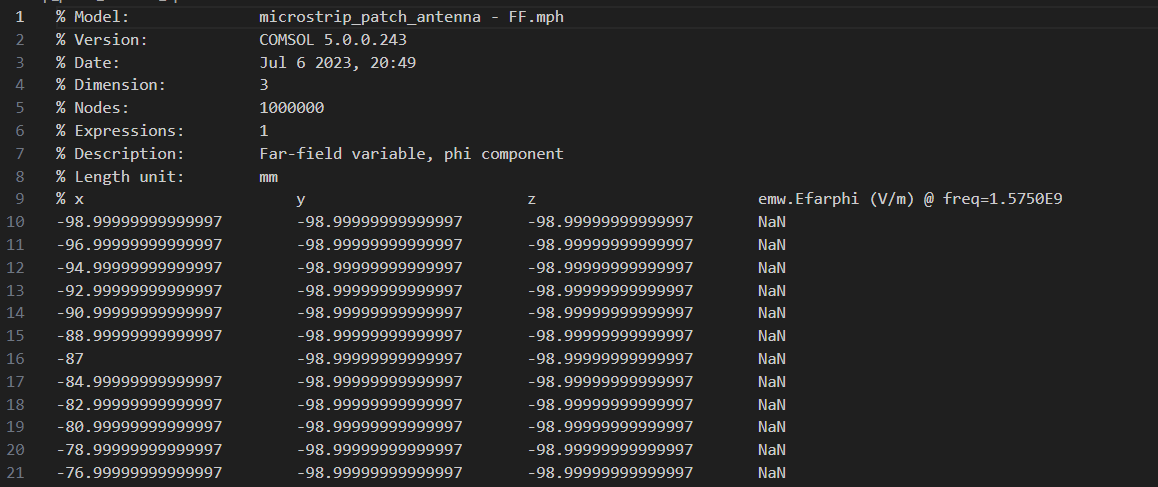
\includegraphics[scale=0.60]{Codigos/Ejemplo fichero COMSOL}
    \caption{Ejemplo de la estructura de un fichero de COMSOL.}
    \label{Ejemplo fichero COMSOL}
\end{figure}

Si nos fijamos, podemos comprobar que las primeras nueve líneas forman parte de la cabecera del fichero. Proporcionando datos relativos a la medición. De la línea diez en adelante, tenemos filas con cuatro valores. Los tres primeros corresponden a las coordenadas a las que se mide el campo. Que en este caso, son cartesianas. Mientras que el último valor corresponde a la medida del campo en esas coordenadas.\\

Esta estructura es siempre la misma independientemente de si medimos el módulo, o una componente concreta del campo. Por lo que las funciones relativas a la lectura del fichero pivotarán siempre entorno a esta estructura.\\

\newpage

Una vez presentado la estructura de fichero con la que vamos a tratar. Lo primero que hemos hecho es una función que lee el fichero línea a línea llamada 
\textit{read\textunderscore{}data} y que tiene la siguiente forma:

\begin{figure}[h]
  \centering
    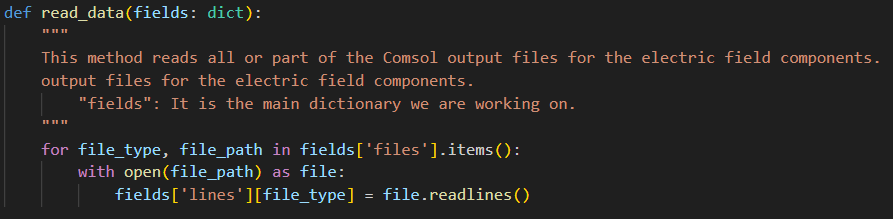
\includegraphics[scale=0.60]{images//Codigos/NFtoNF-esferico_read_data.png}
    \caption{Ejemplo de la estructura de un fichero de COMSOL.}
    \label{Ejemplo fichero COMSOL}
\end{figure}

\newpage
\section{Bibliografía}
\printbibliography
\end{document}

